\subsection{Gruppesamarbejde}
En fælles samarbejdsaftale blev lavet \cref{fig:SAftale}, med aftaler om mødetider og regler omkring brugen af software og værktøjer \cref{fig:4}. Aftalen blev lavet i en skriftlig udgave, fordi så kunne man nemmere referer til arket hvis der kom tvivl om hvad der var aftalt. Samt at alle i gruppen kunne skrive under for at vise at de gik med i hvad der var nedskrevet.

\begin{figure}[ht!]
  \centering
  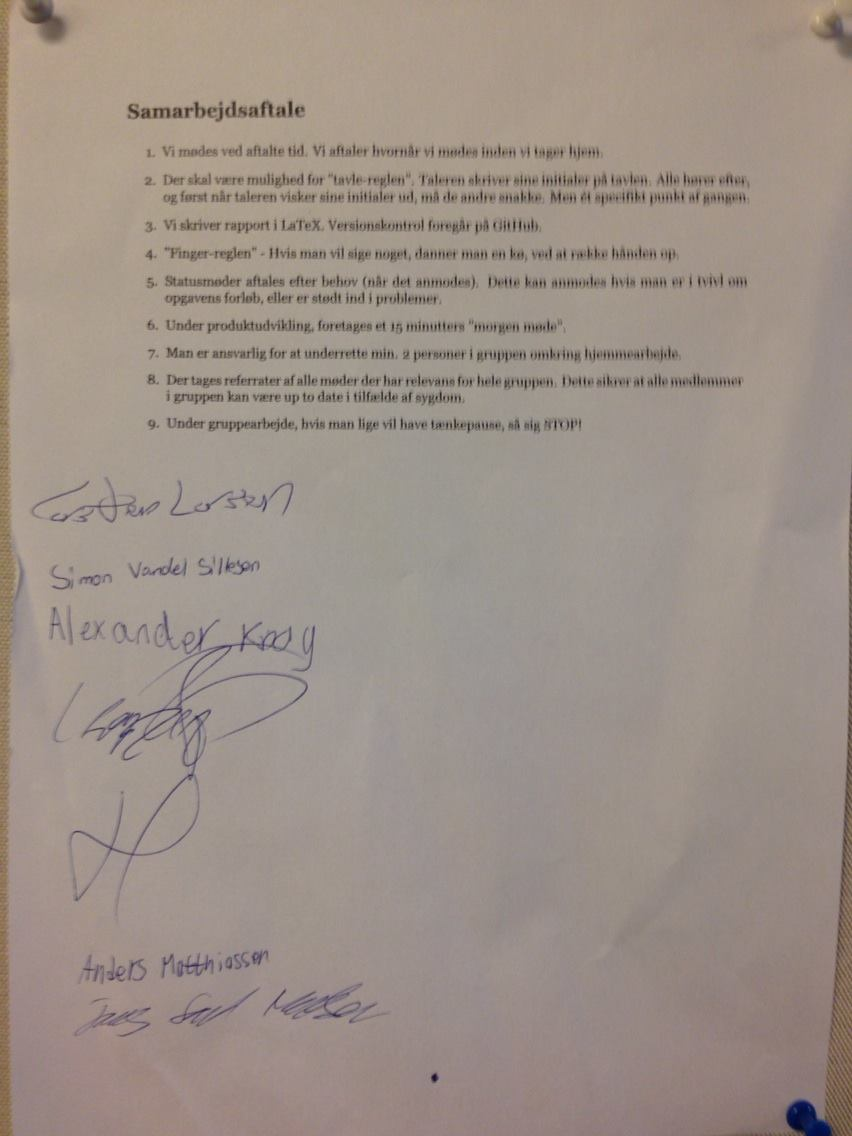
\includegraphics[width=0.5\textwidth]{Images/S_Aftale.jpg}
  \caption{nada}
  \label{fig:SAftale}
\end{figure}

\begin{figure}[ht!]
    \centering
    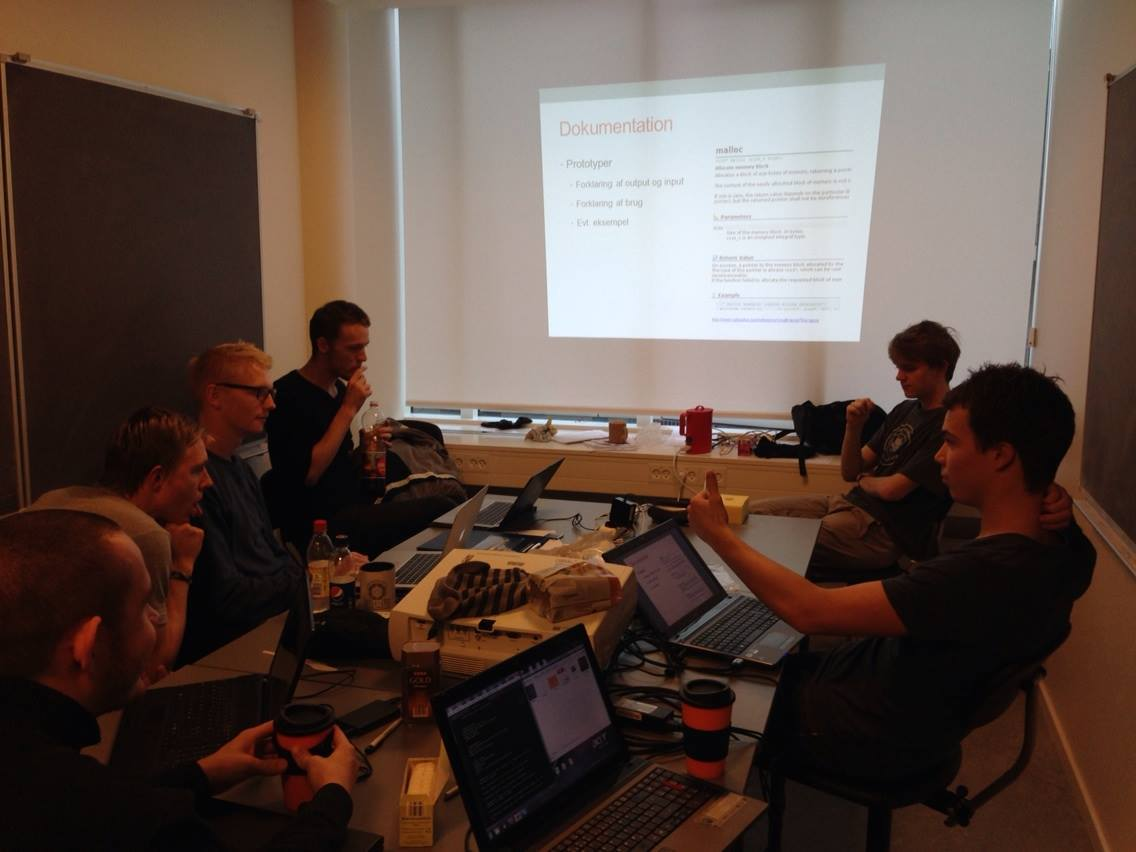
\includegraphics[width=0.5\textwidth]{Images/8.jpg}
    \caption{BAH}
    \label{fig:4}
\end{figure}
Gruppen har været enige om et ambitionsniveau, i forhold til hvad der ar forventet af projektet og kvaliteten af arbejdet. Udenfor projektarbejdet har der været en generel deltagelse i sociale aktiviteter, fordi at det har været godt for at danne sociale relationer til andre grupper, og for at styrke sammenholdet indbyrdes i gruppen. Der blev dog kun deltaget i arrangementer når at projektet var godt med i forhold til tidsplanen. 
Der har som regel været møde med hovedvejleder hver uge, og bivejleder på samme måde, dog med en nedskæring da projektet nærmede sig sin slutning. De opfølgende møder blev aftalt til sidst af hvert møde. Under de daglige møder har der også været en plan, hvis det var at nogle medlemmer ikke mødte op. Hvis et eller flere gruppemedlemmer ikke var mødt op til aftalt tid, og der heller ikke var givet besked, ville gruppemedlemmet blive ringet op af et andet medlem. Hvis opkaldet ikke blev besvaret ville en besked blive vedlagt, og efter en given tidsperiode (et kvarters tids) ville der blive lavet endnu et et opkald i så fald at der ikke var kommunikeret noget tilbage endnu. Når alle var til stede og vores møder begyndte var det velset at man deltog i diskussionerne og at man kom med input. Hvis nogen gruppemedlemmer var meget stille, ville de andre ind spørge til personens mening om det der var emnet for diskussionen. Når der har været en diskussion som har været meget omfattende og gruppemedlemmerne begyndte at afbryde hinanden, blev der taget et "finger system" i brug. Det gik ud på at hvis et gruppemedlem havde noget de ville have sagt i diskussionen, skulle man række en finger i vejret. Den næste der ville sige noget skulle så vise to fingre og den tredje tre finger og så videre. Når den første fik ordet ville han tage fingeren ned og de andre i køen vil vise en finger mindre. På den måde ville der altid kun være en som havde ordet af gangen, og derved blev der ikke brugt for meget tid på at diskutere.

To femte dele inde i projektet da størstedelen af fokussen lå i at skrive analyse var motivationen ikke så høj. Det var grundet i at analysedelen ikke var noget som gruppen fandt videre interessant, dog giv arbejdsmoral op igen da projektet blev mere løsningsorienteret. Under hele projektet blev arbejdsopgaverne fordelt efter interesse og der var aldrig én som alene havde ansvar for en opgave. Det betød at der var mulighed for at delegere en person en opgave, men stadig have flere til at tage ansvar for at opgaven blev lavet.
Gruppen har primært arbejdet i mindre inddelte grupper, fordi at hvis mange tildeles en opgave bliver den ikke nødvendigvis bedre resultater. Også fordi gruppen regelmæssig diskuterede, har det været godt at lave grupperne så en diskussion ikke har stoppet alt arbejdet, men at den gruppe som arbejdede med opgaven kunne tage diskussionen og derved komme frem til afgørelse. Vi har sammensat gruppen efter Belbins team-rolle model, for at gruppen skal kunne begå sig i en bred sammenhæng af situationer. Når der har skulle udeles kritik, blev en begrundelse givet mundtligt og skriftlig i form af noter eller samtaler. Kritikken blev altid modtaget med en begrundelse for hvorfor noget skulle ændres.